\documentclass[twocolumn]{article}
\usepackage[utf8]{inputenc}
\usepackage[english]{babel}
\usepackage{amsmath}	%booklet
\usepackage{hyperref}	%clickable citings, referencing URL via \url{}
\usepackage{siunitx}	%for SI units; see ftp://ftp.dante.de/tex-archive/macros/latex/exptl/siunitx/siunitx.pdf
\usepackage{graphicx} 	%includegraphics
\usepackage{mhchem}		%writing chemical elements with mass numbers
\usepackage[nottoc]{tocbibind}	%references
\usepackage{indentfirst}%indenting first paragraphs

%the command \insertFigure{file} inserts figure with width 0.9*(column width)
%TODO adjust width parameter to get nice results
\newcommand{\insertFigure}[1]{%
   \includegraphics[width=0.9\linewidth]{#1}%
}

\title{K223}
\begin{document}
\maketitle
\newpage
\section{Introduction}
When a nucleus relaxes to the ground state by emitting a $\gamma$-photon, the probability of emitting in a given direction depends on its angle with the nuclear spin axis. If the relaxation happens by emitting two simultaneous photons, these show an angular correlation. This correlation can be measured, which is the goal of the experiment. To that end, first the $\gamma$-ray spectrum of the sample ($\ce{_27^{60}Co}$) was measured, then a FAST-SLOW coincidence circuit was set up (see Figure ~\ref{fig:exp_setup}). 
%TODO $\gamma$-photon is a bad expression, reformulate it
\section{Theory}
Figure \ref{fig:cobalt_scheme} shows the decay scheme of the sample used. The $\ce{_27^{60}Co}$ (half-life $\approx 5.3$ years) decays via $\beta^-$-radiation into $\ce{_28^{60}Ni}$; with highest probability to the $4+$ angular momentum state. %TODO reformulate 4+ angular momentum state, using https://physics.stackexchange.com/questions/338817/photon-spin-in-gamma-decay/340129
The lifetime of these excited $\ce{Ni}$ states are on the order of $\SI{1}{\pico\second}$. 
%TODO reformulate order of picoseconds
Decaying to the ground state follows via emitting one or more $\gamma$ photons. The relaxing process with the largest branching ratio is the $4+ \rightarrow 2+ \rightarrow 0+$ decay, produces two $\gamma$ photons. The corresponding lifetimes are short enough for the emissions to be considered coincidental (from the detecting electronics point of view), and for the assumption that extra-nuclear forces do not cause perturbation in the correlation between the photons.
%TODO write about peaks over natural spectrum appearing in experimental results
\begin{figure}[!h]
\centering
\insertFigure{cobalt_scheme.png}
\caption{Cobalt decay scheme \cite{cobalt_scheme}}
\label{fig:cobalt_scheme}
\end{figure}
\section{Experimental setup}
The design of the apparatus is shown in Figure \ref{fig:exp_setup}. A short description of the purpose and the functioning of the components follows.
\begin{figure}[!h]
\centering
\insertFigure{k223_setup.png}
\caption{Experimental setup \cite{booklet}}
\label{fig:exp_setup}
\end{figure}
\subsection{Detector}
The detectors consist of a crystal scintillator and a photomultiplier. The scintillator absorbs the $\gamma$-ray and re-emits visible light in form of scintillation, which induces electron emission in the photomultiplier via the photoelectric effect. The high voltage provided between the (photo-)cathode and the anode accelerate the electron, which induces an avalanche of electrons by colliding with each of the dynodes, as depicted in Figure \ref{fig:pmt}. As this procedure distorts signal shape, which is required for the measurement of the energy absorbed by the scintillator, the signal on one of the first dynodes is also used as the input for the Single Channel Analyzers \textbf{SCA1} and \textbf{SCA2}.
\begin{figure}[!h]
\centering
\insertFigure{pmt.png} %TODO is the picture allowed to be used? Source: http://wanda.fiu.edu/teaching/courses/Modern_lab_manual/scintillator.html
\caption{Scintillation detector with photomultiplier \cite{pmt}} 
\label{fig:pmt}
\end{figure}
\subsection{The fast coincidence circuit: Constant Fraction Discriminators}
The fast coincidence circuit checks whether the two detected photons come from the same decay process. The constant fraction discriminators modify the signals as seen in Figure \ref{fig:cfd}: an attenuated inverted copy of the input is added to the delayed input signal. The resulting shape crosses the $\SI{0}{\volt}$ line ("zero crossing point"). This point may serve as a time stamp for further processing because the result does not depend on the amplitude.
\par The discriminators have two outputs: while the "fast" output is a negative pulse, the "slow" output is a positive one, hence the latter is used by the fast coincidence unit \textbf{FC}, which does the actual coincidence checking. The output is fed to a gate $\&$ delay generator \textbf{D$^2$-G$^2$}, which delays the gate signal ("trigger" signal): this is required to match the output of the slow coincidence circuit, described in the next section.
%TODO is the original signal truly delayed, or is it the inverted signal? Could provide self-made figure
\begin{figure}[!h]
\centering
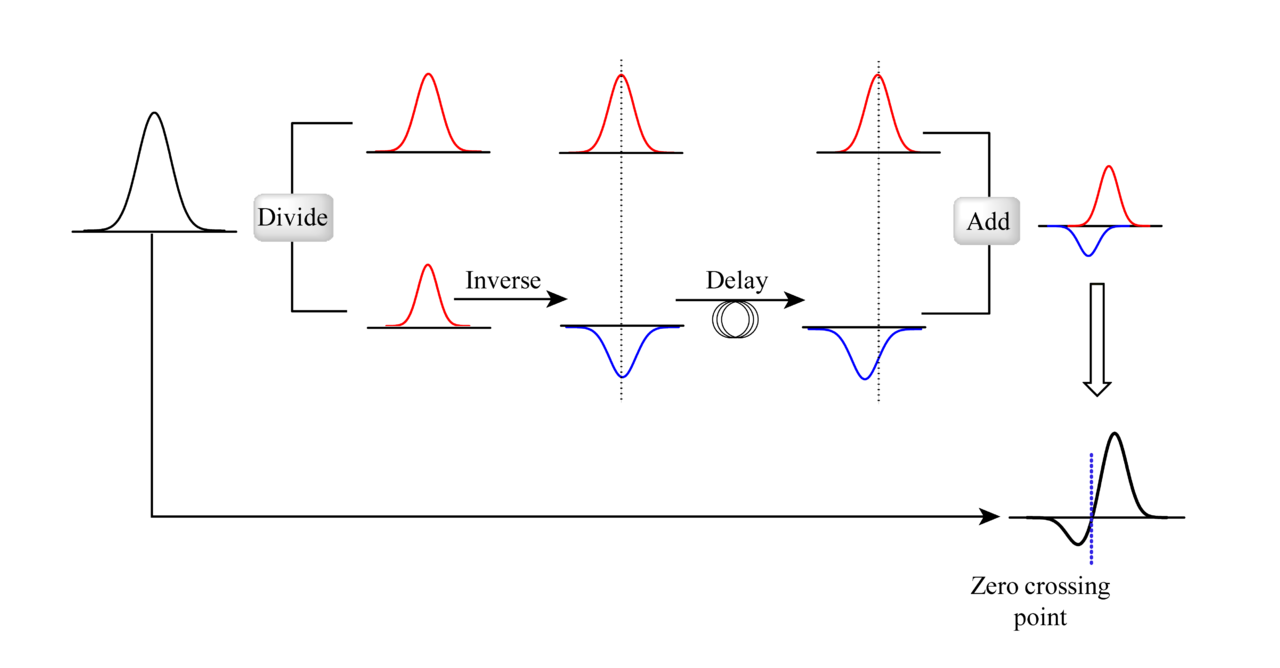
\includegraphics[width=1.2\linewidth]{cfd.png}
\caption{Scintillation detector with photomultiplier \cite{cfd}} 
\label{fig:cfd}
\end{figure}
\subsection{The slow coincidence circuit: Single-Channel Analyzers}
The weak detector signal coming from the earlier dynode is fed through the amplifiers \textbf{A1} and \textbf{A2} first. The analyzers \textbf{SCA1}, \textbf{SCA2} determine whether the amplitudes of the signals --- which are proportional to the energy of the $\gamma$-rays --- fall into an interval with adjustable upper and lower limits.

\section{Procedure}
\subsection{Amplifiers, constant-fraction discriminators}
First the amplifiers \textbf{A$_1$}, \textbf{A$_2$} were adjusted. We changed the gain using an oscilloscope such that the peaks corresponding to different detected photon energy levels don't hit the $\SI{9}{\volt}$ output ceiling of the amplifiers. The result of the adjustment is shown on Figure \ref{fig:amp}. Next we set the threshold of constant-fraction discriminators above the noise level by using the output of the CFD as the trigger for the amplifier signal of the same detector, increasing the threshold until the bright line at $\SI{0}{\volt}$ showing no photon detection (e.g. noise) disappeared. 
%TODO which image, if any, shows the CFD output? Looking for channel 2-trigger.
\subsection{Fast coincidence circuit, prompt curve}
We connected the CFDs' positive outputs to the fast coincidence unit \textbf{FC}, one of them through a delay unit \textbf{D3}. Keeping the resolution time of \textbf{FC} at $\SI{15}{\nano\second}$, we used one of the counter units and changing the delay of \textbf{D3} to measure the coincidental detections as the function of the delay. We measured for $\SI{10}{\second}$ for each delay value.
\begin{figure}
\centering
\insertFigure{./screenshots/SC08.png}
\caption{Well-adjusted signal of the amplifiers on channel 1. A too high gain would cause the highest peaks to flatten as saturation happens before reaching the maximum.} 
\label{fig:amp}
\end{figure}



\iffalse 
\section{useful}
\begin{itemize}
\item Leo 11.3: For technical reasons which we will consider later, it is important to distinguish between fast and slow pulses in an electronics system. Fast signals generally refer to pulses with rise times of a few nanoseconds or less while slow signals have rise times on the order of hundreds of nanosecond or greater. This definition includes both linear and logic signals. Fast pulses are very important for timing applications and high count rates; in these applications it is very important to preserve their rapid rise times throughout the electronics system. Slow pulses, on the other hand, are generally less susceptible to noise and offer better pulse height information for spectroscopy work.
\end{itemize}
\fi

\begin{thebibliography}{9}
%TODO decide upon reference notation (how to format reference works)
\bibitem{booklet}
Booklet.
\bibitem{cobalt_scheme}
R. B. Firestone, Table of Isotopes $8$\textsuperscript{th} edition
 (Wiley, New York, 1996)
 \bibitem{pmt}
 \url{http://wanda.fiu.edu/teaching/courses/Modern_lab_manual/scintillator.html}
\bibitem{cfd}
\url{https://en.wikipedia.org/wiki/Constant_fraction_discriminator#/media/File:Operation_of_a_CFD.png}
%alternative url: https://en.wikipedia.org/wiki/Constant_fraction_discriminator
\end{thebibliography}
\end{document}
